%% ======================================================================
%% Evo2Serve preprint (Zenodo) -- self-contained, no external data files.
%% Build:  pdflatex paper-preprint.tex && pdflatex paper-preprint.tex
%%
%% BEFORE UPLOADING: (1) make the GitHub repository public and add an
%% OSI-approved licence file (for example MIT or Apache-2.0) so that the
%% "Data and Code Availability" statement is true; (2) fill in the three
%% bracketed items in the Declarations section.
%% ======================================================================
\documentclass[10pt,journal,a4paper]{IEEEtran}
\usepackage{cite}
\usepackage{amsmath,amssymb,amsfonts}
\usepackage{booktabs}
\usepackage{graphicx}
\usepackage{textcomp}
\usepackage{xcolor}
\usepackage{array}
\usepackage{tikz}
\usetikzlibrary{arrows.meta,positioning,shapes,shapes.geometric,calc,fit,backgrounds}
\usepackage{pgfplots}
\pgfplotsset{compat=1.18}
\usepgfplotslibrary{groupplots}
\usepackage[hidelinks]{hyperref}
\hypersetup{pdftitle={Evo2Serve: A Web-Deployed Genomic Language Model Service for Zero-Shot Variant Scoring and a Verification Study of Its Scoring Pipeline},pdfauthor={Nandish S Shet, Thippeswamy S, Vishwaradhya A C, Jeevan A M, Nandini K S}}

%% ---- figure data (inlined from docs/analysis/figure_data.tex) ----
%% composition of the assay set and of the calibration slice
\def\assayFUNC{2821}\def\assayINT{249}\def\assayLOF{823}
\def\sliceFUNC{400}\def\sliceINT{0}\def\sliceLOF{100}

%% position coverage of the assayed region and of the calibration slice
\def\coverageAll{(0.0000,453) (0.0250,452) (0.0500,287) (0.0750,0) (0.1000,0) (0.1250,303) (0.1500,0) (0.1750,0) (0.2000,133) (0.2250,448) (0.2500,0) (0.2750,311) (0.3000,306) (0.3250,0) (0.3500,0) (0.3750,0) (0.4000,0) (0.4250,0) (0.4500,0) (0.4750,0) (0.5000,0) (0.5250,0) (0.5500,0) (0.5750,0) (0.6000,0) (0.6250,0) (0.6500,0) (0.6750,0) (0.7000,0) (0.7250,0) (0.7500,393) (0.7750,203) (0.8000,0) (0.8250,0) (0.8500,0) (0.8750,292) (0.9000,0) (0.9250,0) (0.9500,0) (0.9750,312) (1.0000,0)}
\def\coverageSlice{(0.0000,0) (0.0250,0) (0.0500,0) (0.0750,0) (0.1000,0) (0.1250,0) (0.1500,0) (0.1750,0) (0.2000,0) (0.2250,0) (0.2500,0) (0.2750,0) (0.3000,0) (0.3250,0) (0.3500,0) (0.3750,0) (0.4000,0) (0.4250,0) (0.4500,0) (0.4750,0) (0.5000,0) (0.5250,0) (0.5500,0) (0.5750,0) (0.6000,0) (0.6250,0) (0.6500,0) (0.6750,0) (0.7000,0) (0.7250,0) (0.7500,0) (0.7750,0) (0.8000,0) (0.8250,0) (0.8500,0) (0.8750,188) (0.9000,0) (0.9250,0) (0.9500,0) (0.9750,312) (1.0000,0)}
\def\coverageLo{41197722}
\def\coverageHi{41276135}

%% ROC curves of the reference predictors on the calibration slice
\def\rocCADD{(0.0000,0.0000) (0.0000,0.0300) (0.0000,0.0700) (0.0000,0.1700) (0.0025,0.1900) (0.0075,0.1900) (0.0200,0.2000) (0.0200,0.2300) (0.0300,0.2300) (0.0300,0.2400) (0.0375,0.2400) (0.0400,0.2400) (0.0425,0.2500) (0.0450,0.2500) (0.0525,0.2500) (0.0625,0.2500) (0.0650,0.2500) (0.0750,0.2500) (0.0750,0.2700) (0.0825,0.2800) (0.0875,0.2800) (0.0925,0.2900) (0.0950,0.3000) (0.1025,0.3000) (0.1125,0.3200) (0.1150,0.3200) (0.1175,0.3300) (0.1225,0.3400) (0.1225,0.3500) (0.1350,0.3500) (0.1375,0.4000) (0.1425,0.4200) (0.1525,0.4300) (0.1650,0.4700) (0.1675,0.4700) (0.1725,0.4800) (0.1750,0.4900) (0.1800,0.4900) (0.1925,0.5000) (0.1950,0.5100) (0.2050,0.5200) (0.2125,0.5300) (0.2175,0.5600) (0.2350,0.5700) (0.2450,0.6100) (0.2500,0.6400) (0.2550,0.6400) (0.2675,0.6700) (0.2700,0.6900) (0.2750,0.7000) (0.2825,0.7100) (0.2925,0.7400) (0.2975,0.7400) (0.3100,0.7600) (0.3150,0.7600) (0.3200,0.7700) (0.3225,0.7900) (0.3250,0.7900) (0.3325,0.8200) (0.3425,0.8400) (0.3500,0.8600) (0.3625,0.8600) (0.3700,0.8700) (0.3800,0.8700) (0.3825,0.8800) (0.3850,0.9000) (0.3900,0.9000) (0.4025,0.9000) (0.4050,0.9100) (0.4100,0.9200) (0.4225,0.9300) (0.4275,0.9300) (0.4300,0.9300) (0.4350,0.9300) (0.4375,0.9300) (0.4425,0.9300) (0.4450,0.9300) (0.4600,0.9300) (0.5150,0.9300) (0.5200,0.9300) (0.5725,0.9300) (0.5725,0.9400) (0.5800,0.9400) (0.5800,0.9500) (0.6025,0.9500) (0.6025,0.9600) (0.6075,0.9600) (0.6225,0.9600) (0.6250,0.9700) (0.6325,0.9700) (0.6325,0.9800) (0.6600,0.9800) (0.6650,0.9800) (0.6925,0.9800) (0.6975,0.9800) (0.7025,0.9800) (0.7075,0.9800) (0.7125,0.9800) (0.7175,0.9800) (0.7725,0.9800) (0.7775,0.9800) (0.9250,0.9800) (0.9250,0.9900) (0.9375,0.9900) (0.9375,1.0000) (0.9925,1.0000) (0.9975,1.0000) (1.0000,1.0000)}
\def\rocaGVD{(0.0000,0.0000) (0.0000,0.0476) (0.0049,0.0794) (0.0049,0.1746) (0.0098,0.1746) (0.0098,0.2222) (0.0146,0.2381) (0.0146,0.2857) (0.0341,0.2857) (0.0341,0.3810) (0.0341,0.4286) (0.0390,0.4286) (0.0390,0.4444) (0.0390,0.4762) (0.0390,0.4921) (0.0488,0.4921) (0.0488,0.5238) (0.0585,0.5238) (0.0585,0.5556) (0.0634,0.5714) (0.0634,0.6349) (0.0732,0.6349) (0.0732,0.6667) (0.0732,0.7302) (0.0780,0.7302) (0.0829,0.7460) (0.0829,0.7619) (0.1024,0.7619) (0.1122,0.7619) (0.1171,0.7619) (0.1268,0.7619) (0.1317,0.7619) (0.1317,0.7778) (0.1415,0.7778) (0.1463,0.7778) (0.1610,0.7778) (0.1707,0.7778) (0.1756,0.7778) (0.1756,0.7937) (0.1951,0.7937) (0.1951,0.8095) (0.2049,0.8095) (0.2146,0.8095) (0.2195,0.8095) (0.2195,0.8254) (0.2244,0.8254) (0.2341,0.8254) (0.2390,0.8571) (0.2488,0.8571) (0.2488,0.9048) (0.2585,0.9048) (0.2829,0.9048) (0.2927,0.9048) (0.3268,0.9048) (0.3317,0.9048) (0.3512,0.9048) (0.3561,0.9048) (0.3707,0.9048) (0.3805,0.9048) (0.3951,0.9048) (0.4146,0.9048) (0.4439,0.9048) (0.4634,0.9048) (0.5171,0.9048) (0.5171,0.9206) (0.5220,0.9206) (0.5220,0.9365) (0.5366,0.9365) (0.5512,0.9365) (0.5561,0.9365) (0.5707,0.9365) (0.5951,0.9365) (0.6049,0.9365) (0.6244,0.9365) (0.6341,0.9365) (0.6585,0.9365) (0.6585,0.9524) (0.6732,0.9524) (0.6878,0.9524) (0.7122,0.9524) (0.7268,0.9683) (0.7317,0.9683) (0.7463,0.9683) (0.7463,0.9841) (0.7561,0.9841) (0.7756,0.9841) (0.8000,0.9841) (0.8390,0.9841) (0.8488,0.9841) (0.8585,0.9841) (0.8585,1.0000) (0.8976,1.0000) (0.9073,1.0000) (0.9220,1.0000) (0.9268,1.0000) (0.9366,1.0000) (0.9463,1.0000) (0.9707,1.0000) (1.0000,1.0000)}
\def\rocphyloP{(0.0000,0.0000) (0.0400,0.1700) (0.1100,0.3300) (0.1175,0.3300) (0.2025,0.5200) (0.3950,0.8800) (0.4100,0.8800) (0.4400,0.8800) (0.4475,0.8800) (0.4500,0.9000) (0.4575,0.9000) (0.4600,0.9200) (0.4900,0.9200) (0.5025,0.9300) (0.5550,0.9300) (0.5650,0.9500) (0.5675,0.9700) (0.5900,0.9700) (0.6050,0.9700) (0.7325,0.9700) (0.7450,0.9800) (0.7825,0.9800) (0.7875,0.9900) (0.8400,0.9900) (0.8450,1.0000) (0.9725,1.0000) (0.9775,1.0000) (1.0000,1.0000)}
\def\rocPolyPhen2{(0.0000,0.0000) (0.0098,0.0000) (0.0341,0.0159) (0.0488,0.0476) (0.0537,0.0476) (0.0537,0.0794) (0.0878,0.1270) (0.1024,0.1429) (0.1073,0.1587) (0.1317,0.1746) (0.1317,0.1905) (0.1415,0.2381) (0.1561,0.2381) (0.1707,0.3175) (0.1756,0.3175) (0.1902,0.3333) (0.1951,0.3333) (0.1951,0.3810) (0.1951,0.3968) (0.2049,0.3968) (0.2293,0.4127) (0.2537,0.4444) (0.2585,0.4444) (0.2780,0.4921) (0.2829,0.5714) (0.2878,0.5714) (0.2976,0.5873) (0.2976,0.6349) (0.3024,0.6349) (0.3512,0.6349) (0.3512,0.6508) (0.3610,0.6508) (0.3610,0.6984) (0.3854,0.7143) (0.4000,0.7143) (0.4049,0.7143) (0.4146,0.7143) (0.4195,0.7143) (0.4244,0.7302) (0.4293,0.7302) (0.4341,0.7460) (0.4390,0.7460) (0.4634,0.7460) (0.4683,0.7460) (0.4683,0.7619) (0.4732,0.7619) (0.4829,0.7619) (0.4829,0.8254) (0.4976,0.8254) (0.5024,0.8254) (0.5268,0.8571) (0.5366,0.8571) (0.5366,0.8730) (0.5512,0.8730) (0.5610,0.8730) (0.5756,0.8730) (0.5756,0.8889) (0.5854,0.8889) (0.6098,0.8889) (0.6098,0.9048) (0.6195,0.9048) (0.6390,0.9048) (0.6439,0.9048) (0.6439,0.9206) (0.6537,0.9206) (0.6634,0.9206) (0.6732,0.9206) (0.6829,0.9206) (0.7171,0.9206) (0.7268,0.9206) (0.7366,0.9206) (0.7463,0.9206) (0.7512,0.9365) (0.7854,0.9365) (0.7951,0.9365) (0.8000,0.9365) (0.8146,0.9365) (0.8244,0.9365) (0.8341,0.9365) (0.8585,0.9365) (0.8585,0.9524) (0.8780,0.9524) (0.8927,0.9524) (0.8927,0.9683) (0.9122,0.9683) (0.9122,0.9841) (0.9415,0.9841) (0.9415,1.0000) (0.9561,1.0000) (0.9659,1.0000) (0.9805,1.0000) (1.0000,1.0000)}
\def\rocSIFT{(0.0000,0.0000) (0.6878,1.0000) (0.7463,1.0000) (0.7805,1.0000) (0.8049,1.0000) (0.8244,1.0000) (0.8341,1.0000) (0.8537,1.0000) (0.8634,1.0000) (0.8683,1.0000) (0.8878,1.0000) (0.9073,1.0000) (0.9220,1.0000) (0.9317,1.0000) (0.9463,1.0000) (0.9610,1.0000) (0.9902,1.0000) (1.0000,1.0000)}

%% confidence heuristic sampled from the source constants
\def\confLOF{(-0.004000,1.0000) (-0.003850,1.0000) (-0.003700,1.0000) (-0.003550,1.0000) (-0.003400,1.0000) (-0.003250,1.0000) (-0.003100,1.0000) (-0.002950,1.0000) (-0.002800,1.0000) (-0.002650,1.0000) (-0.002500,1.0000) (-0.002350,0.9459) (-0.002200,0.8468) (-0.002050,0.7478) (-0.001900,0.6487) (-0.001750,0.5496) (-0.001600,0.4506) (-0.001450,0.3515) (-0.001300,0.2524) (-0.001150,0.1533) (-0.001000,0.0543)}
\def\confFUNC{(-0.000850,0.0753) (-0.000700,0.2416) (-0.000550,0.4080) (-0.000400,0.5743) (-0.000250,0.7407) (-0.000100,0.9071) (0.000050,1.0000) (0.000200,1.0000) (0.000350,1.0000) (0.000500,1.0000) (0.000650,1.0000) (0.000800,1.0000) (0.000950,1.0000) (0.001100,1.0000) (0.001250,1.0000) (0.001400,1.0000) (0.001550,1.0000) (0.001700,1.0000) (0.001850,1.0000) (0.002000,1.0000)}
\def\confTau{-0.0009178519}
\def\confSigLOF{0.0015140239}
\def\confSigFUNC{0.0009016589}
%% ---- end of figure data ----

\begin{document}

\title{Evo2Serve: A Web-Deployed Genomic Language Model Service for Zero-Shot Variant Scoring and a Verification Study of Its Scoring Pipeline}

\author{\IEEEauthorblockN{Nandish S Shet\IEEEauthorrefmark{1}, Thippeswamy S\IEEEauthorrefmark{1}, Vishwaradhya A C\IEEEauthorrefmark{1}, Jeevan A M\IEEEauthorrefmark{1}, and Dr.~Nandini K S\IEEEauthorrefmark{2}\IEEEauthorrefmark{3}}\\
\IEEEauthorblockA{Department of Artificial Intelligence and Data Science,\\Don Bosco Institute of Technology, Bengaluru, Karnataka, India}\\
\IEEEauthorblockA{\IEEEauthorrefmark{1}Student authors \quad \IEEEauthorrefmark{2}Associate Professor and faculty guide \quad \IEEEauthorrefmark{3}Corresponding author\\
\textit{Preprint, version 1. This manuscript has not been peer reviewed.}}}

\maketitle

%% ----------------------------------------------------------------------
\begin{abstract}
Genomic language models such as Evo~2 can score the effect of a DNA change without task-specific training, but the label shown to a user also depends on a software contract (context window, coordinates, edit rules, threshold and request validation) that is rarely examined. We describe Evo2Serve, a web application that scores single-nucleotide variants, deletions, insertions and deletion--insertions of up to 500 bases with Evo~2-7B on a serverless NVIDIA H100 GPU, applies a threshold calibrated on BRCA1 saturation genome editing data, and shows the result beside ClinVar. We then verify the deployed pipeline without running the model. The 500-variant calibration slice contains 100 loss-of-function and 400 functional variants but covers only 10.69\% of the assayed interval. On that slice, reference predictors reach AUROCs from 0.53 (gnomAD frequency) to 0.88 (Align-GVGD), CADD 0.79, with bootstrap half-widths of about 0.03 to 0.07 for most. The deployed endpoint fetches an 8193-base window where calibration used 8192. The GRCh37 and GRCh38 assemblies differ by a constant 1{,}847{,}983 bases at BRCA1, and the request carries no reference allele that could expose a coordinate from the wrong assembly. Across 55 request cases, the Pydantic and Zod validators conform on 43 and 47, disagree on 6, and both mishandle 7, including assembly and chromosome strings with separator characters that both accept. We list eight defects with proposed repairs. Latency and throughput were not measured. The tool is for research and education and is not a clinical classifier.
\end{abstract}

\begin{IEEEkeywords}
Variant effect prediction, genomic language model, Evo~2, BRCA1, ClinVar, web application, serverless GPU, software verification, bioinformatics.
\end{IEEEkeywords}

%% ----------------------------------------------------------------------
\section{Introduction}
A genomic language model can be asked a simple question: how plausible does this stretch of DNA look, with and without a given change? Evo~2, which was trained on a broad collection of genomes and not on human variation data, answers it at single-nucleotide resolution over contexts of up to one million bases, and on a saturation genome editing benchmark for \emph{BRCA1} it reached a zero-shot AUROC of 0.9037 over 3{,}893 variants~\cite{brixi2026evo2,findlay2018brca1}. Such a result justifies interest in the model. It does not, however, justify any particular label attached to a particular coordinate entered by a particular person.

Between the benchmark and the user sits a software layer. A person picks an assembly and a gene, reads a sequence, and types a position and an alternate allele. The application must resolve that position against a reference genome, retrieve a context window, build the edited sequence, obtain two model scores, subtract them, compare the difference with a threshold and draw a label. Each step can fail without any visible sign. A coordinate taken from the wrong assembly, for example, yields a confident answer about a different base. The interpretation standards that clinical laboratories follow treat computational predictions as supporting evidence only~\cite{richards2015acmg,pejaver2022svi}, so a tool that emits the words ``likely pathogenic'' owes its users an account of how that word was produced.

This paper presents Evo2Serve, a browser-based service built around Evo~2-7B, and reports a verification study of its deployed scoring pipeline. The study was carried out in an environment without a graphics processor, so it concerns everything around the model (data, window, coordinates, validation, decision rule) and not the model's own accuracy. The contributions are:
\begin{itemize}
\item an end-to-end system that connects public genome databases to Evo~2-7B on a serverless H100 through a two-stage authenticated and validated request path, supporting four edit types and displaying each prediction beside ClinVar;
\item a formal specification of the deployed scoring contract: window construction, the four edit operations, the score difference, the threshold decision rule and the confidence heuristic;
\item a characterisation of the BRCA1 calibration data and a reproducible reference-predictor envelope for the 500-variant slice used to set the threshold, with bootstrap intervals;
\item verification of the window contract (8193 versus 8192 bases), of assembly handling (a constant offset of 1{,}847{,}983 bases between GRCh37 and GRCh38 at BRCA1 and its consequences), and of request validation over 55 cases executed against both validators; and
\item a list of eight defects and improvements, each traced to a script that a reader can re-run.
\end{itemize}

Section~\ref{sec:related} reviews related work. Section~\ref{sec:system} describes the system and Section~\ref{sec:contract} states the scoring contract and its calibration. Section~\ref{sec:design} sets out the evaluation design, Section~\ref{sec:results} reports the results, and Sections~\ref{sec:discussion} and~\ref{sec:limits} discuss them and their limits. Section~\ref{sec:conclusion} concludes.

%% ----------------------------------------------------------------------
\section{Related Work}
\label{sec:related}

\textit{Variant effect predictors.} SIFT estimates tolerance of an amino-acid change from conservation across homologous sequences~\cite{ng2001sift}, PolyPhen-2 combines alignment and structural features~\cite{adzhubei2010polyphen2}, and CADD integrates many genomic annotations into one deleteriousness score for any variant~\cite{rentzsch2019cadd}. The Ensembl Variant Effect Predictor wraps such tools in a standard annotation pipeline~\cite{mclaren2016vep}. Protein language models extend the idea to the proteome; AlphaMissense, for instance, scores missense variants at proteome scale~\cite{cheng2023alphamissense}, and protein language models such as ESM-2 learn from protein sequences at scale~\cite{lin2023esm2}. Most of these methods are limited to coding changes or depend on precomputed annotations, which is why a model that scores an arbitrary edited sequence is attractive.

\textit{Genomic language models.} Models that read nucleotide sequences directly include DNABERT-2~\cite{zhou2024dnabert2}, Nucleotide Transformer~\cite{dallatorre2024nt}, Enformer~\cite{avsec2021enformer}, Borzoi~\cite{linder2025borzoi} and GPN-MSA, which adds multispecies alignments~\cite{benegas2025gpnmsa}. Evo showed that a single model can be trained on genomes at scale~\cite{nguyen2024evo}. Evo~2 extends this to 7B and 40B parameters and a one-million-token context using the StripedHyena~2 multi-hybrid architecture~\cite{brixi2025stripedhyena2,brixi2026evo2}. In the Evo~2 paper, zero-shot Evo~2-7B is reported at AUROC 0.9037 on the full BRCA1 benchmark against 0.8763 for CADD, while a supervised classifier fitted on Evo~2 embeddings does better still~\cite{brixi2026evo2}. These numbers describe the model on the whole assay; they say nothing about a service built on a small calibration subset.

\textit{Cautions from the literature.} Likelihoods from sequence-only models can reflect phylogenetic structure rather than function, and correcting for it improves variant effect prediction~\cite{pugh2025likelihood}. A classical phylogenetic method has been reported to outperform large protein language models~\cite{prillo2024siterm}, and variant effect predictors as a group show ancestry-dependent behaviour~\cite{pathak2024ancestry}. On the clinical side, the ACMG/AMP guidelines give computational evidence at most supporting weight~\cite{richards2015acmg}, and the ClinGen Sequence Variant Interpretation Working Group has described how a computational score must be calibrated locally before it can be mapped to evidence strength~\cite{pejaver2022svi}.

\textit{Deployed interpretation services.} VarSome aggregates annotations from many sources behind one query box~\cite{kopanos2019varsome}, and MobiDetails presents curated variant evidence online~\cite{baux2021mobidetails}. The Evo~2 authors provide interactive tools for generation and scoring with the model~\cite{brixi2026evo2}, and EVEE serves variant effect predictions derived from genomic foundation model embeddings~\cite{pearce2026evee}. Evo2Serve is not an annotation aggregator. It exposes one model's score for an arbitrary user-entered edit and converts it to a binary label through its own threshold, so the label is only as sound as the window, coordinate handling and calibration behind it. Those three are the subject of the verification study.

%% ----------------------------------------------------------------------
\section{System Architecture}
\label{sec:system}

Evo2Serve has three tiers (Fig.~\ref{fig:arch}). A browser client renders the interface and performs all public data lookups. A Next.js API route checks the user's session and validates each analysis request. A FastAPI endpoint hosted on Modal verifies a second token, fetches the context window and runs Evo~2-7B on an NVIDIA H100.

\begin{figure*}[!t]
\centering
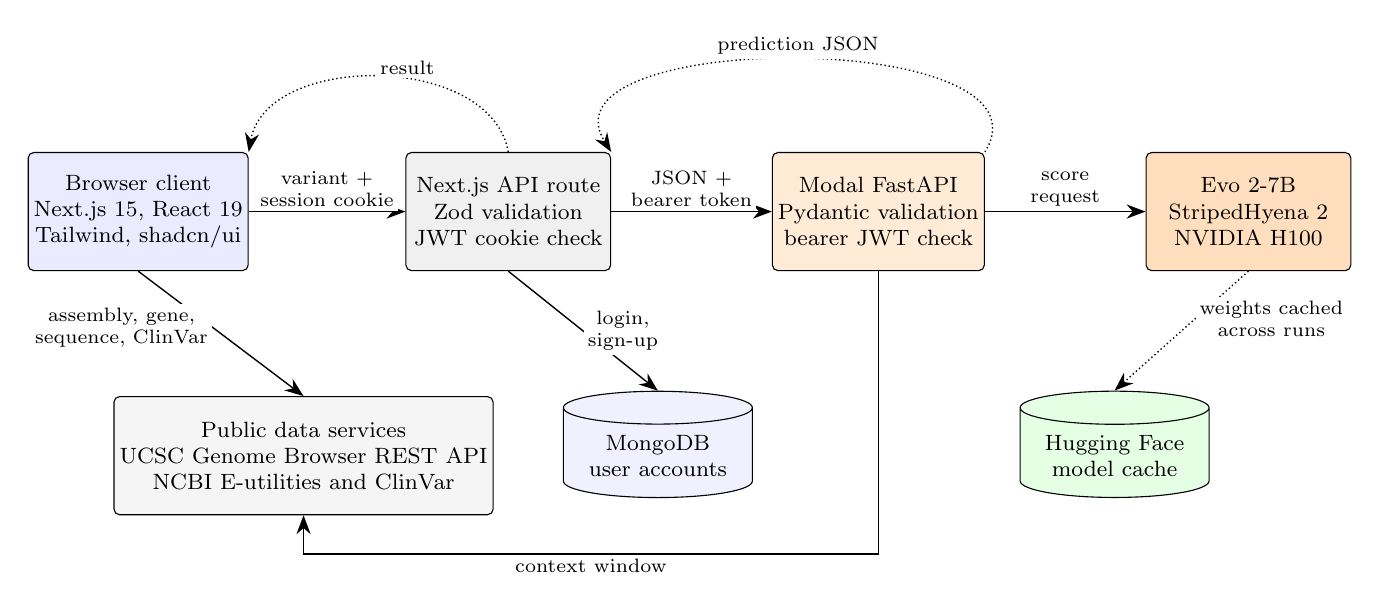
\begin{tikzpicture}[>=Stealth,font=\footnotesize,
  box/.style={rectangle,draw,rounded corners=2pt,minimum width=2.6cm,minimum height=1.5cm,align=center,inner sep=2pt,line width=0.4pt},
  store/.style={cylinder,draw,shape border rotate=90,aspect=0.22,minimum width=2.4cm,minimum height=1.35cm,align=center,inner sep=2pt,line width=0.4pt},
  lbl/.style={font=\scriptsize,align=center,inner sep=1.5pt,fill=white},
  edge/.style={-{Stealth[length=2.4mm]},line width=0.5pt},
  back/.style={-{Stealth[length=2.4mm]},line width=0.5pt,densely dotted}]
\node[box,fill=blue!8] (ui) at (0,0) {Browser client\\Next.js 15, React 19\\Tailwind, shadcn/ui};
\node[box,fill=gray!12] (route) at (4.7,0) {Next.js API route\\Zod validation\\JWT cookie check};
\node[box,fill=orange!16] (api) at (9.4,0) {Modal FastAPI\\Pydantic validation\\bearer JWT check};
\node[box,fill=orange!26] (gpu) at (14.1,0) {Evo 2-7B\\StripedHyena 2\\NVIDIA H100};
\node[store,fill=green!10] (cache) at (12.4,-3.1) {Hugging Face\\model cache};
\node[box,fill=gray!8,minimum width=4.6cm] (pub) at (2.1,-3.1) {Public data services\\UCSC Genome Browser REST API\\NCBI E-utilities and ClinVar};
\node[store,fill=blue!6] (db) at (6.6,-3.1) {MongoDB\\user accounts};
\draw[edge] (ui.east) -- node[lbl,above,pos=0.5]{variant +\\session cookie} (route.west);
\draw[edge] (route.east) -- node[lbl,above,pos=0.5]{JSON +\\bearer token} (api.west);
\draw[edge] (api.east) -- node[lbl,above,pos=0.5]{score\\request} (gpu.west);
\draw[back] (gpu.south) -- node[lbl,right,pos=0.40]{weights cached\\across runs} (cache.north);
\draw[back] (api.north east) to[out=58,in=122] node[lbl,above,pos=0.5]{prediction JSON} (route.north east);
\draw[back] (route.north) to[out=100,in=80] node[lbl,above,pos=0.42]{result} (ui.north east);
\draw[edge] (ui.south) -- node[lbl,left,pos=0.45]{assembly, gene,\\sequence, ClinVar} (pub.north);
\draw[edge] (api.south) -- (9.4,-4.35) -- node[lbl,below,pos=0.5]{context window} (2.1,-4.35) -- (pub.south);
\draw[edge] (route.south) -- node[lbl,right,pos=0.5]{login,\\sign-up} (db.north);
\end{tikzpicture}
\caption{Request path of Evo2Serve. The browser performs the public lookups and posts analysis requests to the Next.js route, which checks the session and forwards a bearer token. The Modal endpoint verifies the token, fetches the context window from UCSC, scores the reference and edited sequences and returns the result. Solid arrows are requests and dotted arrows are responses.}
\label{fig:arch}
\end{figure*}

\subsection{Front End}
The client is a Next.js~15 application written in TypeScript with React~19, Tailwind CSS and shadcn/ui components. It requests the list of human assemblies from UCSC~\cite{lee2022ucsc,lee2020ucscapi}, with hg38 as the default, and lets the user browse chromosomes or search genes through NCBI services. A gene view shows the reference sequence (at most 10{,}000 displayed bases), gene details, a variant entry panel and a table of up to 20 ClinVar records~\cite{landrum2024clinvar}, retrieved with the \texttt{chrpos38} search field for hg38 and \texttt{chrpos37} for hg19. Clicking a base fills the position and reference allele of the variant form. For a ClinVar record, one click submits the variant to the endpoint and opens a comparison view that places the model's label beside the ClinVar classification.

\subsection{Back End}
The back end is a Python application on Modal built from a CUDA~12.6.3 image with PyTorch~2.7.1, FlashAttention~2.8.0 and the official Evo~2 package. The model is loaded once per container, model weights live on a persistent Hugging Face cache volume, and the analysis function is exposed as a FastAPI POST endpoint. Modal is configured for at most three H100 containers, a 120-second scale-down window and two retries. These are configuration values, not measured capacity. The same code base contains the calibration routine of Section~\ref{sec:contract}, which runs as a separate Modal GPU job. Table~\ref{tab:stack} summarises the stack and the constants visible in the source.

\begin{table}[!t]
\caption{Implementation stack and constants visible in the source.}
\label{tab:stack}
\centering
\footnotesize
\begin{tabular}{@{}ll@{}}
\toprule
Layer & Choice or constant \\
\midrule
Model, window & Evo 2-7B, 8192-base window parameter \\
Serving & Modal, FastAPI, H100, 3 containers max \\
Front end & Next.js 15, React 19, TypeScript, Tailwind \\
Authentication & HS256 JWT in cookie; bearer token to GPU tier \\
Validation & Zod (web route), Pydantic (GPU tier) \\
Edit limits & deletion and insertion length $\le 500$ bases \\
Threshold & $\tau=-0.0009178519$ \\
Class spreads & $\sigma_{\mathrm{LOF}}=0.0015140239$, $\sigma_{\mathrm{FUNC}}=0.0009016589$ \\
Public data & UCSC REST API, NCBI E-utilities, ClinVar \\
\bottomrule
\end{tabular}
\end{table}

\subsection{Authentication and Request Validation}
Users register and sign in with an e-mail address and a password, which is stored as a bcrypt hash in MongoDB. Sign-in issues an HS256 JSON Web Token in an HTTP-only cookie valid for seven days. The Next.js route rejects a request without a valid cookie with HTTP~401, validates the JSON body with a Zod schema, and forwards the body with the token as a bearer header. The Modal endpoint independently verifies the token and validates the body with a Pydantic model before it touches the GPU. The two schemas were written separately by hand, and Section~\ref{sec:res-validation} measures how far they agree.

%% ----------------------------------------------------------------------
\section{Scoring Contract and Calibration}
\label{sec:contract}

\subsection{Context Window}
Let $p$ be the 1-based coordinate of a substitution, of the anchor base of an insertion, or of the first affected base of a deletion or deletion--insertion (delins), let $n$ be the number of deleted bases and $q$ the inserted string. The window centre is $c=p$ for a substitution or insertion and $c=p+\lfloor(n-1)/2\rfloor$ for a deletion or delins, which keeps the flanks balanced. With the window parameter $W=8192$ and half-width $h=\lfloor W/2\rfloor=4096$, the backend asks UCSC for the half-open interval
\begin{equation}
s=\max(0,\,c-1-h), \qquad e=c-1+h+1.
\label{eq:window}
\end{equation}
The start is clipped at zero, and the end is not clipped locally. Because both halves of the interval include the central base, an interior request returns $e-s=W+1=8193$ bases. If $w$ is the returned upper-case sequence, the zero-based offset of the edit within it is $r=p-1-s$.

\subsection{Edit Operations}
For an alternate base $a$, the edited sequence for each supported edit type is (Fig.~\ref{fig:edits})
\begin{align}
w^{\mathrm{SNV}} &= w_{0:r} + a + w_{r+1:}, \label{eq:snv}\\
w^{\mathrm{DEL}} &= w_{0:r} + w_{r+n:}, \label{eq:del}\\
w^{\mathrm{INS}} &= w_{0:r+1} + q + w_{r+1:}, \label{eq:ins}\\
w^{\mathrm{DELINS}} &= w_{0:r} + q + w_{r+n:}. \label{eq:delins}
\end{align}
Deleted and inserted lengths are limited to 500 bases, and inserted strings are restricted to A, C, G and T.

\begin{figure}[!t]
\centering
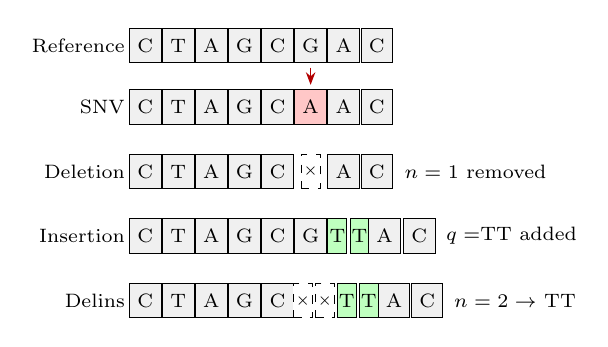
\begin{tikzpicture}[font=\scriptsize,
  cell/.style={rectangle,draw,minimum width=0.40cm,minimum height=0.44cm,align=center,inner sep=0pt,line width=0.35pt},
  ctx/.style={cell,fill=gray!12},
  altc/.style={cell,fill=red!22},
  nar/.style={rectangle,draw,minimum width=0.24cm,minimum height=0.44cm,align=center,inner sep=0pt,line width=0.35pt},
  insc/.style={nar,fill=green!25},
  gapc/.style={nar,dashed,fill=white},
  rowlbl/.style={font=\scriptsize,anchor=east,inner sep=1.5pt},
  note/.style={font=\scriptsize,anchor=west,inner sep=1pt}]
\node[rowlbl] at (-0.20,0) {Reference};
\node[ctx] at (0,0) {C};  \node[ctx] at (0.42,0) {T};
\node[ctx] at (0.84,0) {A}; \node[ctx] at (1.26,0) {G};
\node[ctx] at (1.68,0) {C}; \node[ctx] at (2.10,0) {G};
\node[ctx] at (2.52,0) {A}; \node[ctx] at (2.94,0) {C};
\node[rowlbl] at (-0.20,-0.78) {SNV};
\node[ctx] at (0,-0.78) {C};  \node[ctx] at (0.42,-0.78) {T};
\node[ctx] at (0.84,-0.78) {A}; \node[ctx] at (1.26,-0.78) {G};
\node[ctx] at (1.68,-0.78) {C}; \node[altc] at (2.10,-0.78) {A};
\node[ctx] at (2.52,-0.78) {A}; \node[ctx] at (2.94,-0.78) {C};
\draw[-{Stealth[length=1.6mm]},red!70!black,line width=0.5pt] (2.10,-0.28) -- (2.10,-0.50);
\node[rowlbl] at (-0.20,-1.60) {Deletion};
\node[ctx] at (0,-1.60) {C};  \node[ctx] at (0.42,-1.60) {T};
\node[ctx] at (0.84,-1.60) {A}; \node[ctx] at (1.26,-1.60) {G};
\node[ctx] at (1.68,-1.60) {C}; \node[gapc] at (2.10,-1.60) {\tiny$\times$};
\node[ctx] at (2.52,-1.60) {A}; \node[ctx] at (2.94,-1.60) {C};
\node[note] at (3.25,-1.60) {$n=1$ removed};
\node[rowlbl] at (-0.20,-2.42) {Insertion};
\node[ctx] at (0,-2.42) {C};  \node[ctx] at (0.42,-2.42) {T};
\node[ctx] at (0.84,-2.42) {A}; \node[ctx] at (1.26,-2.42) {G};
\node[ctx] at (1.68,-2.42) {C}; \node[ctx] at (2.10,-2.42) {G};
\node[insc] at (2.44,-2.42) {T}; \node[insc] at (2.72,-2.42) {T};
\node[ctx] at (3.04,-2.42) {A}; \node[ctx] at (3.48,-2.42) {C};
\node[note] at (3.78,-2.42) {$q=$TT added};
\node[rowlbl] at (-0.20,-3.24) {Delins};
\node[ctx] at (0,-3.24) {C};  \node[ctx] at (0.42,-3.24) {T};
\node[ctx] at (0.84,-3.24) {A}; \node[ctx] at (1.26,-3.24) {G};
\node[ctx] at (1.68,-3.24) {C};
\node[gapc] at (2.00,-3.24) {\tiny$\times$}; \node[gapc] at (2.28,-3.24) {\tiny$\times$};
\node[insc] at (2.56,-3.24) {T}; \node[insc] at (2.84,-3.24) {T};
\node[ctx] at (3.16,-3.24) {A}; \node[ctx] at (3.58,-3.24) {C};
\node[note] at (3.88,-3.24) {$n=2\rightarrow$ TT};
\end{tikzpicture}
\caption{The four edit operations applied by the backend. Context bases are grey, the substituted base is red and inserted bases are green. A crossed cell is a removed base.}
\label{fig:edits}
\end{figure}

\subsection{Score Difference}
Let $S(\cdot)$ be the mean per-base natural-log likelihood that the Evo~2 scoring routine returns for a sequence. Because it is an average over the positions of that sequence, the reference and edited scores are averages over different numbers of positions whenever an edit changes the length. The score difference is
\begin{equation}
\Delta = S(w^{\mathrm{var}}) - S(w^{\mathrm{ref}}),
\label{eq:delta}
\end{equation}
and a negative $\Delta$ means that the model finds the edited sequence less plausible~\cite{brixi2026evo2}. The endpoint scores the reference and the edited sequence on every request, which is two forward passes, and keeps no cache between requests.

\subsection{Threshold Calibration}
The decision threshold was fitted on the BRCA1 saturation genome editing data~\cite{findlay2018brca1}, following the zero-shot protocol of the Evo~2 authors~\cite{brixi2026evo2}. Non-functional variants form the positive (loss-of-function, LOF) class, and functional plus intermediate variants form the negative class. The calibration routine scores a window around each variant taken from the GRCh37 chromosome~17 sequence, builds $\Delta$, and selects the operating point that maximises Youden's index on the ROC curve of $-\Delta$~\cite{hanley1982roc,youden1950index}:
\begin{equation}
J(t)=\mathrm{TPR}(t)-\mathrm{FPR}(t), \qquad t^{\star}=\arg\max_t J(t).
\label{eq:youden}
\end{equation}
The routine uses a window of $[p-1-h,\,p-1+h)$, which is 8192 bases with the variant at offset 4096, and it scores identical reference windows only once. Because one GPU run over the whole assay is costly, the routine was applied to the first 500 rows of the data. The resulting constants (Table~\ref{tab:stack}) are compiled into the endpoint; the per-variant output of the run that produced them was not archived.

\subsection{Decision Rule and Confidence}
The deployed endpoint labels a request with the fixed threshold $\tau=-0.0009178519$ as
\begin{equation}
\mathrm{label}=\begin{cases}
\text{Likely pathogenic}, & \Delta < \tau,\\
\text{Likely benign}, & \text{otherwise},
\end{cases}
\label{eq:call}
\end{equation}
and reports a confidence value that grows with the distance of $\Delta$ from $\tau$, scaled by the spread of the predicted class and capped at one:
\begin{equation}
\mathrm{conf}=\min\!\left(1,\frac{|\Delta-\tau|}{\sigma_{\mathrm{class}}}\right),
\label{eq:conf}
\end{equation}
with $\sigma_{\mathrm{LOF}}=0.0015140239$ on the pathogenic side and $\sigma_{\mathrm{FUNC}}=0.0009016589$ on the benign side. Figure~\ref{fig:conf} plots the function. It is a bounded distance and not a probability, and nothing in the repository shows it to be calibrated. Deletions, insertions and delins reuse the substitution constants because no indel-specific calibration exists, and their responses carry a provisional flag.

\begin{figure}[!t]
\centering
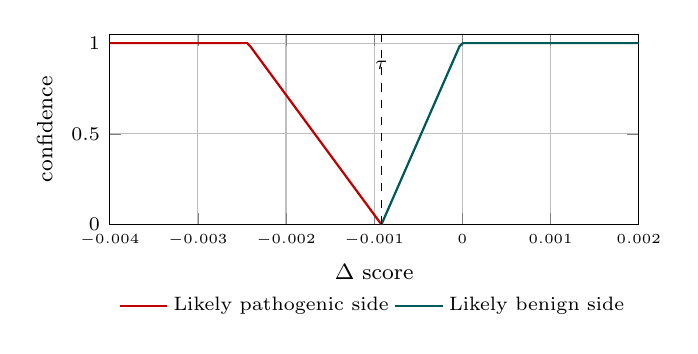
\begin{tikzpicture}
\begin{axis}[width=8.3cm,height=4.0cm,grid=major,
 xlabel={$\Delta$ score},ylabel={confidence},
 xmin=-0.004,xmax=0.002,ymin=0,ymax=1.05,
 legend style={font=\scriptsize,at={(0.5,-0.32)},anchor=north,legend columns=2,draw=none},
 tick label style={font=\scriptsize},label style={font=\footnotesize},
 scaled x ticks=false,xtick={-0.004,-0.003,-0.002,-0.001,0,0.001,0.002},
 xticklabel style={/pgf/number format/fixed,/pgf/number format/precision=3,font=\tiny}]
\addplot[thick,red!75!black,domain=-0.004:\confTau,samples=80] {min(1,abs(x-\confTau)/\confSigLOF)};
\addplot[thick,teal!70!black,domain=\confTau:0.002,samples=80] {min(1,abs(x-\confTau)/\confSigFUNC)};
\addplot[dashed,black,line width=0.4pt] coordinates {(\confTau,0) (\confTau,1.05)};
\node[font=\scriptsize,anchor=south] at (axis cs:\confTau,0.80) {$\tau$};
\legend{Likely pathogenic side,Likely benign side}
\end{axis}
\end{tikzpicture}
\caption{The confidence heuristic of Eq.~\eqref{eq:conf}: distance of $\Delta$ from the threshold $\tau$, divided by the spread of the predicted class and capped at one.}
\label{fig:conf}
\end{figure}

%% ----------------------------------------------------------------------
\section{Evaluation Design}
\label{sec:design}

The verification study examines five aspects of the deployed pipeline. It separates what was measured from what could not be, and every result below is produced by a script in the repository (folder \texttt{docs/analysis}).

\textit{Calibration data.} We read the supplementary workbook of the BRCA1 assay, recompute its class composition, and characterise the 500-row slice used for the threshold: class counts, position coverage, reference-base agreement with the GRCh37 chromosome~17 sequence, and window content.

\textit{Reference envelope.} The workbook carries precomputed scores for CADD, PolyPhen-2, SIFT, Align-GVGD, phyloP and gnomAD allele frequency. We evaluate them on the identical 500 rows, with the same labels and the same Youden procedure as the calibration routine. Intervals are 95\% percentile bootstrap intervals from 2{,}000 resamples stratified by class, with a fixed seed.

\textit{Window and assembly contract.} We recompute both window rules for all 500 calibration positions, and we align GRCh37 and GRCh38 across the BRCA1 locus on conserved anchors. The derived offset is checked against the NCBI Gene model for BRCA1 and against the paired coordinates of live ClinVar records.

\textit{Request validation.} We generated 55 request cases covering every discriminating field, both boundaries of each numeric limit, the 500-base length cap and malformed values. Each case carries an expected verdict derived from the request specification and the documented limits, not from either implementation. We execute the cases against the real Pydantic model imported from the backend and the real Zod schema extracted from the route handler.

\textit{Scoring contract.} We import the deployed window and edit functions and exercise them with a stand-in scorer, a third-order Markov background model estimated from the chromosome~17 sequence and reduced with the same mean. The stand-in is not Evo~2. The arithmetic of the contract (lengths, offsets, decision rule, confidence) does not depend on which model supplies the two likelihoods.

Evo~2 was not run in the verification environment, so no Evo~2 score was generated and no accuracy is claimed for the deployed service. Latency and throughput were not measured.

%% ----------------------------------------------------------------------
\section{Results}
\label{sec:results}

\subsection{Calibration Data}
\label{sec:res-data}
The workbook contains 3{,}893 variants: 2{,}821 functional (72.46\%), 249 intermediate (6.40\%) and 823 non-functional (21.14\%). These shares reproduce the 72.5\%, 6.4\% and 21.1\% reported for the assay~\cite{findlay2018brca1}. All 500 reference bases of the calibration rows agree with the GRCh37 sequence, and none of the 500 calibration windows contains an ambiguous base.

The calibration slice has 100 non-functional and 400 functional variants (intermediate variants: none), a positive rate of 20.0\%, which is close to that of the whole assay. It is, however, spatially concentrated (Fig.~\ref{fig:slice}, Table~\ref{tab:slice}). Its positions span 8{,}380 of the 78{,}413 assayed bases, or 10.69\%, and it touches 168 distinct transcript positions and 41 amino-acid positions. The class mix also changes along the slice: the first 250 rows contain 30 non-functional variants and the last 250 contain 70. A threshold fitted on it therefore describes a small region of one gene whose composition is not uniform.

\begin{figure}[!t]
\centering
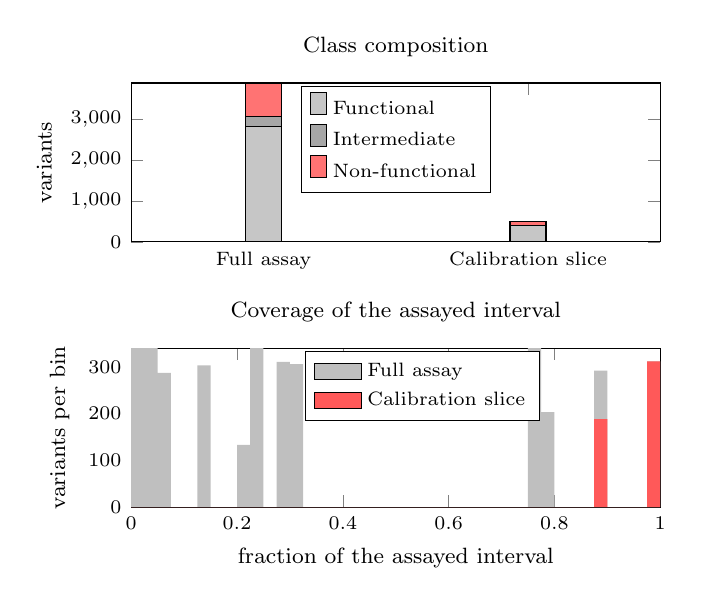
\begin{tikzpicture}
\begin{groupplot}[width=8.3cm,height=3.6cm,
 group style={group size=1 by 2, vertical sep=1.35cm},
 xlabel style={font=\footnotesize},ylabel style={font=\footnotesize},
 tick label style={font=\scriptsize},
 legend style={font=\scriptsize,at={(0.98,0.98)},anchor=north east}]
\nextgroupplot[
 title={Class composition},title style={font=\footnotesize},
 ybar stacked,bar width=13pt,
 symbolic x coords={Full assay,Calibration slice},
 xtick=data,ylabel={variants},
 ymin=0,ymax=3900,enlarge x limits=0.5,legend cell align=left,
 legend style={at={(0.5,0.98)},anchor=north}]
\addplot[fill=gray!45] coordinates {(Full assay,\assayFUNC) (Calibration slice,\sliceFUNC)};
\addplot[fill=gray!70] coordinates {(Full assay,\assayINT) (Calibration slice,\sliceINT)};
\addplot[fill=red!55] coordinates {(Full assay,\assayLOF) (Calibration slice,\sliceLOF)};
\legend{Functional,Intermediate,Non-functional}
\nextgroupplot[
 title={Coverage of the assayed interval},title style={font=\footnotesize},
 xlabel={fraction of the assayed interval},ylabel={variants per bin},
 xmin=0,xmax=1,ymin=0,ymax=340,
 legend cell align={left},legend style={font=\scriptsize,at={(0.55,0.98)},anchor=north}]
\addplot[ybar interval,fill=gray!50,draw=none,mark=none,area legend] coordinates {\coverageAll};
\addplot[ybar interval,fill=red!65,draw=none,mark=none,area legend] coordinates {\coverageSlice};
\legend{Full assay,Calibration slice}
\end{groupplot}
\end{tikzpicture}
\caption{The BRCA1 calibration data. Top: class composition of the full assay and of the 500-variant slice. Bottom: variants per bin along the assayed interval; the slice occupies two clusters near one end of the interval.}
\label{fig:slice}
\end{figure}

\begin{table}[!t]
\caption{BRCA1 data used for calibration.}
\label{tab:slice}
\centering
\footnotesize
\begin{tabular}{@{}lrr@{}}
\toprule
Property & Full assay & Slice \\
\midrule
Variants & 3{,}893 & 500 \\
Non-functional (LOF) & 823 (21.14\%) & 100 (20.0\%) \\
Functional + intermediate & 3{,}070 (78.86\%) & 400 (80.0\%) \\
LOF in first / last 250 rows & --- & 30 / 70 \\
Transcript positions & 1{,}326 & 168 \\
Amino-acid positions & 326 & 41 \\
Span (GRCh37) & 78{,}413\,bp & 8{,}380\,bp \\
Share of assayed interval & 100\% & 10.69\% \\
Reference base matches GRCh37 & --- & 500/500 \\
Window GC, mean (range) & --- & 0.462 (0.427--0.485) \\
Distinct reference windows & 1{,}326 & 168 \\
\bottomrule
\end{tabular}
\end{table}

\subsection{Reference-Predictor Envelope}
\label{sec:res-baselines}
Table~\ref{tab:baselines} and Fig.~\ref{fig:roc} give the AUROC of the precomputed predictors on the identical 500 rows. The column $n$ is the number of slice variants for which a score exists; the missense-specific predictors lack scores for the 232 non-missense rows. Align-GVGD is the strongest at 0.878, CADD reaches 0.791 and phyloP 0.777, whereas PolyPhen-2 (0.683) and SIFT (0.656) are weaker, and gnomAD allele frequency is close to chance (0.530), as expected for variants that were engineered and not drawn from a population. The 95\% bootstrap half-widths are about 0.03 to 0.07 for the predictors with real signal (0.02 for allele frequency), so neighbouring predictors are not reliably ordered on 500 variants.

\begin{table}[!t]
\caption{Reference predictors on the 500-variant calibration slice (loss of function positive). AUROC with 95\% bootstrap intervals; sensitivity and specificity at the Youden operating point. $n$: rows with a score. These values measure the scores stored in the workbook, not the original tools.}
\label{tab:baselines}
\centering
\footnotesize
\setlength{\tabcolsep}{4pt}
\begin{tabular}{@{}lcrrrr@{}}
\toprule
Predictor & $n$ & AUROC & 95\% CI & Sens. & Spec. \\
\midrule
Align-GVGD & 268 & 0.878 & 0.821--0.929 & 0.762 & 0.917 \\
CADD & 500 & 0.791 & 0.750--0.835 & 0.900 & 0.615 \\
phyloP (mammalian) & 500 & 0.777 & 0.729--0.820 & 0.880 & 0.605 \\
PolyPhen-2 & 268 & 0.683 & 0.613--0.750 & 0.825 & 0.517 \\
SIFT & 268 & 0.656 & 0.624--0.688 & 1.000 & 0.312 \\
gnomAD AF & 500 & 0.530 & 0.506--0.553 & 0.960 & 0.100 \\
\midrule
Random & 500 & 0.500 & --- & --- & --- \\
\bottomrule
\end{tabular}
\end{table}

\begin{figure}[!t]
\centering
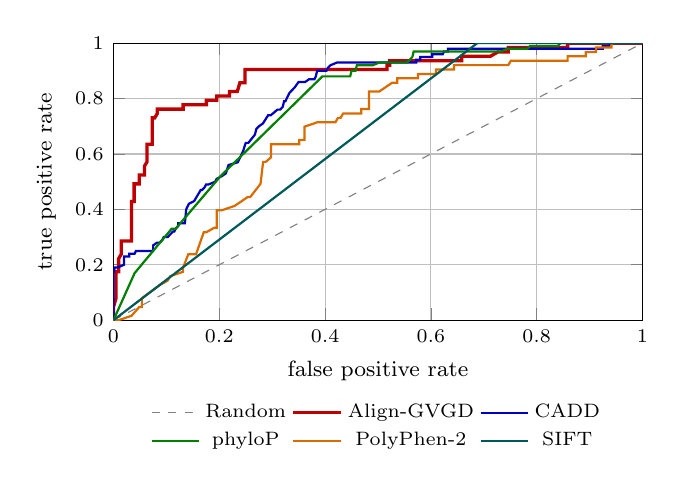
\begin{tikzpicture}
\begin{axis}[width=8.3cm,height=5.1cm,grid=major,
 xlabel={false positive rate},ylabel={true positive rate},
 xmin=0,xmax=1,ymin=0,ymax=1,
 legend style={font=\scriptsize,at={(0.5,-0.26)},anchor=north,legend columns=3,draw=none},
 tick label style={font=\scriptsize},label style={font=\footnotesize}]
\addplot[dashed,gray,line width=0.4pt] coordinates {(0,0) (1,1)};
\addplot[very thick,red!75!black] coordinates {\rocaGVD};
\addplot[thick,blue!75!black] coordinates {\rocCADD};
\addplot[thick,green!50!black] coordinates {\rocphyloP};
\addplot[thick,orange!85!black] coordinates {\rocPolyPhen2};
\addplot[thick,teal!70!black] coordinates {\rocSIFT};
\legend{Random,Align-GVGD,CADD,phyloP,PolyPhen-2,SIFT}
\end{axis}
\end{tikzpicture}
\caption{ROC curves of the reference predictors on the 500-variant calibration slice, with loss of function as the positive class.}
\label{fig:roc}
\end{figure}

Table~\ref{tab:evo2} lists the published zero-shot results of the Evo~2 paper on the \emph{full} 3{,}893-variant assay~\cite{brixi2026evo2}. Those figures belong to the Evo~2 paper and not to this deployment. The slice is a harder test than the whole assay for at least one predictor: CADD scores 0.8763 on all variants but 0.791 on the slice, a drop of about 0.09 that exceeds the gap between most pairs of predictors in Table~\ref{tab:baselines}. The tracks also differ (phyloP over 100 vertebrates in the published table, a mammalian track in the workbook). Comparisons between the slice and the full assay should therefore be made with the restriction stated.

\begin{table}[!t]
\caption{Published zero-shot results on the full BRCA1 assay (823 LOF, 3{,}070 other), quoted from the Evo~2 paper~\cite{brixi2026evo2}.}
\label{tab:evo2}
\centering
\footnotesize
\begin{tabular}{@{}lrr@{}}
\toprule
Model & AUROC & AUPRC \\
\midrule
Evo 2-7B & 0.9037 & 0.7326 \\
Evo 2-40B & 0.9011 & 0.6771 \\
CADD & 0.8763 & 0.7295 \\
GPN-MSA & 0.8628 & 0.6498 \\
phyloP (100 vertebrates) & 0.8113 & 0.4945 \\
Nucleotide Transformer & 0.5496 & 0.2847 \\
Evo 1 & 0.4972 & 0.2158 \\
\bottomrule
\end{tabular}
\end{table}

A single calibration run of the deployed model on the 500 slice rows yielded an AUROC of about 0.73. We report it as a preliminary figure only: the per-variant scores of that run were not archived, it cannot be re-derived from the repository, and it has not been validated or independently reproduced. We therefore do not place it in Table~\ref{tab:baselines} and draw no conclusion from it.

\subsection{Window Contract}
\label{sec:res-window}
The calibration routine and the deployed endpoint build different windows (Fig.~\ref{fig:window}). The routine takes $[p-1-h,\,p-1+h)$, 8192 bases, and the endpoint takes the interval of Eq.~\eqref{eq:window}, 8193 bases, which is the calibration window plus one base at the 3$'$ end. For all 500 calibration positions the endpoint window equals the calibration window except for that final base, the edit offset is 4096 in both, and no window is clipped at a chromosome boundary. The mean in Eq.~\eqref{eq:delta} is therefore taken over one more position in deployment than in calibration. The effect on $\Delta$ is expected to be small, but it cannot be quantified without running the model, so we record the mismatch as a defect rather than a measured error.

\begin{figure*}[!t]
\centering
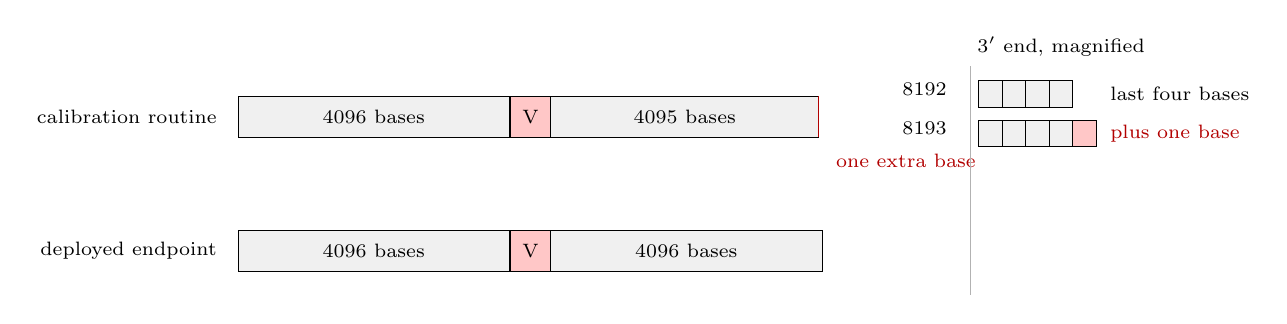
\begin{tikzpicture}[font=\scriptsize,
  seg/.style={rectangle,draw,minimum height=0.52cm,align=center,inner sep=1.5pt,line width=0.4pt},
  ctxs/.style={seg,fill=gray!12},
  vars/.style={seg,fill=red!22,minimum width=0.52cm},
  zc/.style={rectangle,draw,minimum width=0.30cm,minimum height=0.34cm,align=center,inner sep=0pt,line width=0.35pt},
  zx/.style={zc,fill=gray!12},
  zr/.style={zc,fill=red!22},
  note/.style={font=\scriptsize,anchor=west,inner sep=1pt}]
\draw[ctxs] (0,0.55) rectangle (3.45,1.07);
\node at (1.72,0.81) {4096 bases};
\draw[vars] (3.45,0.55) rectangle (3.97,1.07);
\node at (3.71,0.81) {V};
\draw[ctxs] (3.97,0.55) rectangle (7.37,1.07);
\node at (5.67,0.81) {4095 bases};
\draw[line width=0.5pt,red!70!black] (7.37,0.55) -- (7.37,1.07);
\node[note,red!70!black] at (7.55,0.25) {one extra base};
\node[anchor=east,font=\scriptsize] at (-0.15,0.81) {calibration routine};
\draw[ctxs] (0,-1.15) rectangle (3.45,-0.63);
\node at (1.72,-0.89) {4096 bases};
\draw[vars] (3.45,-1.15) rectangle (3.97,-0.63);
\node at (3.71,-0.89) {V};
\draw[ctxs] (3.97,-1.15) rectangle (7.42,-0.63);
\node at (5.69,-0.89) {4096 bases};
\node[anchor=east,font=\scriptsize] at (-0.15,-0.89) {deployed endpoint};
\draw[gray!60,line width=0.4pt] (9.30,-1.45) -- (9.30,1.45);
\node[font=\scriptsize,align=center] at (10.45,1.70) {3$'$ end, magnified};
\node[font=\scriptsize,anchor=east] at (9.12,1.16) {8192};
\foreach \i in {0,1,2,3} \node[zx] at (9.55+\i*0.30,1.10) {};
\node[font=\scriptsize,anchor=east] at (9.12,0.66) {8193};
\foreach \i in {0,1,2,3} \node[zx] at (9.55+\i*0.30,0.60) {};
\node[zr] at (9.55+4*0.30,0.60) {};
\node[font=\scriptsize,anchor=west] at (10.95,1.10) {last four bases};
\node[font=\scriptsize,anchor=west,red!70!black] at (10.95,0.60) {plus one base};
\end{tikzpicture}
\caption{The deployed context window and the calibration window. Both place the variant V at offset 4096, so the upstream context is identical. The endpoint adds one base at the 3$'$ end, giving 8193 bases where the calibration routine used 8192. The inset magnifies the 3$'$ end.}
\label{fig:window}
\end{figure*}

\subsection{Assembly Offset and Its Consequences}
\label{sec:res-assembly}
The calibration data use GRCh37 coordinates, the interface defaults to GRCh38 and offers every human assembly that UCSC lists, and nothing on the request path converts coordinates between assemblies. Aligning the two assemblies across \emph{BRCA1} on 681 conserved anchors gives a constant offset of 1{,}847{,}983 bases (GRCh38 minus GRCh37). All 680 consecutive anchor pairs are free of insertions and deletions, so the offset does not drift across the gene. It is consistent with the NCBI Gene model, which places \emph{BRCA1} at 43{,}044{,}294--43{,}170{,}326 on GRCh38, and with the 290 live ClinVar \emph{BRCA1} records that carry both coordinates, where the difference is 1{,}847{,}983 in every record (Table~\ref{tab:assembly}).

The consequences follow from this. If a correct GRCh37 coordinate is lifted by the offset, the reference base matches the assay for all 500 calibration variants and the 8192-base windows are identical, so for BRCA1 the sequence scored is the sequence intended. The risk lies in an unlifted coordinate. The shipped example request (hg38, chr17:43{,}119{,}628) has reference base T. The same numeric position in hg19 holds C, the lifted hg19 position 41{,}271{,}645 holds T, and the hg19 and hg38 windows at the same number agree at only 25.2\% of positions, which is the level expected by chance (Fig.~\ref{fig:assembly}). Because the request carries no reference allele, the service cannot notice such a mismatch and returns a label with a confidence value either way. The coordinate and not the sequence is the weak point for this gene, and a gene with indels between assemblies would also show a changing offset.

\begin{figure}[!t]
\centering
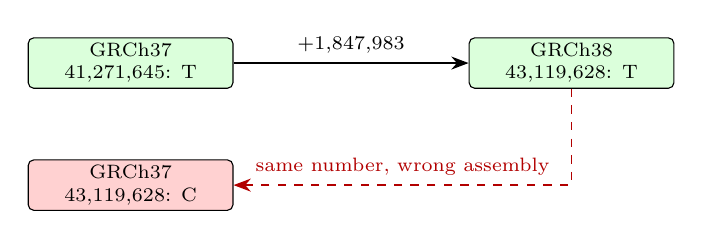
\begin{tikzpicture}[font=\scriptsize,
  ax/.style={-{Stealth[length=2.2mm]},line width=0.5pt},
  b/.style={rectangle,draw,rounded corners=2pt,minimum height=0.55cm,align=center,inner sep=2pt,line width=0.4pt}]
\node[b,fill=green!14,minimum width=2.6cm] (g19) at (0,0) {GRCh37\\41{,}271{,}645: T};
\node[b,fill=green!14,minimum width=2.6cm] (g38) at (5.6,0) {GRCh38\\43{,}119{,}628: T};
\node[b,fill=red!18,minimum width=2.6cm] (wrong) at (0,-1.55) {GRCh37\\43{,}119{,}628: C};
\draw[ax] (g19.east) -- node[above,font=\scriptsize]{$+1{,}847{,}983$} (g38.west);
\draw[ax,red!70!black,dashed] (g38.south) -- (5.6,-1.55) -- node[above,font=\scriptsize,text=red!70!black]{same number, wrong assembly} (wrong.east);
\end{tikzpicture}
\caption{The shipped example request at the BRCA1 locus. The GRCh38 position 43{,}119{,}628 and the GRCh37 position 41{,}271{,}645 name the same base, T. Reading the GRCh38 number as a GRCh37 coordinate (dashed) gives C, and the request carries no reference allele that would reveal the mismatch.}
\label{fig:assembly}
\end{figure}

\begin{table}[!t]
\caption{Assembly checks at the BRCA1 locus.}
\label{tab:assembly}
\centering
\footnotesize
\begin{tabular}{@{}lr@{}}
\toprule
Quantity & Value \\
\midrule
Conserved anchors aligned & 681 \\
Consecutive anchor pairs without an indel & 680 of 680 \\
GRCh38 minus GRCh37 offset (all anchors) & 1{,}847{,}983 \\
ClinVar records with both coordinates & 290 \\
Distinct offsets among those records & 1 \\
Calibration bases correct after lifting & 500/500 \\
Windows identical after lifting & median 0 differing bases \\
Example, same numeric coordinate in hg19 & C (hg38 is T) \\
Example, lifted hg19 coordinate & T at 41{,}271{,}645 \\
\bottomrule
\end{tabular}
\end{table}

The browser adds a second path to the same failure. ClinVar is searched in the assembly the user selected, but the position forwarded to the endpoint is the \texttt{location\_sort} field of the record summary. Among 300 live \emph{BRCA1} records, this field equals the GRCh38 start in 293 and the GRCh37 start in none. With hg19 selected, the application therefore locates the correct record and then submits its GRCh38 position together with the hg19 genome name.

\subsection{Request-Validation Conformance}
\label{sec:res-validation}
Table~\ref{tab:validation} summarises the 55 cases. The Pydantic model conforms to the expected verdict on 43 and the Zod schema on 47. Both conform on 42 cases and the layers give different verdicts on 6.

\begin{table}[!t]
\caption{Conformance of the two request validators over 55 cases.}
\label{tab:validation}
\centering
\footnotesize
\begin{tabular}{@{}lr@{}}
\toprule
Outcome & Cases \\
\midrule
Pydantic conforming & 43 \\
Zod conforming & 47 \\
Both conforming & 42 \\
Pydantic wrong, Zod right & 5 \\
Zod wrong, Pydantic right & 1 \\
Both wrong & 7 \\
\midrule
Layers disagree & 6 \\
\bottomrule
\end{tabular}
\end{table}

\textit{Disagreements.} In five cases Pydantic accepts a request that the specification rejects and Zod correctly refuses: a zero position, a negative position, an empty genome, an empty chromosome, and an insertion of 495 bases followed by six spaces. In the sixth, a lowercase alternate base, the specification and Pydantic accept and Zod refuses, which is a false rejection. Zod measures the length cap on the raw string whereas Pydantic first removes spaces and newlines. Since Zod rejects in all six, none of them passes through the browser route to the GPU, but a caller holding a valid token can post directly to the endpoint and reach the five weaker cases.

\textit{Both wrong.} Seven cases are mishandled by both layers. Six are assembly or chromosome values containing a UCSC parameter separator (semicolon), a newline, a slash or a space; both layers accept them although the specification forbids them. The backend interpolates these two fields into the UCSC query string, where parameters are themselves separated by semicolons~\cite{lee2020ucscapi}, so a crafted value can inject extra parameters into an outgoing request. The seventh is a whitespace-padded alternate base, which the specification accepts but both layers reject.

\subsection{Scoring-Contract Behaviour}
\label{sec:res-contract}
Run with the stand-in scorer, a 3-base deletion produced scored sequences of 8193 and 8190 bases and a 3-base insertion produced 8193 and 8196 bases, as Eqs.~\eqref{eq:del} and \eqref{eq:ins} require. Indel responses carried the provisional flag and the substitution response did not. These checks concern lengths, offsets and flags and say nothing about Evo~2 scores.

One behaviour is independent of any model. A substitution whose alternate base equals the reference base is accepted, produces an edited sequence identical to the reference, and therefore gives $\Delta=0$ exactly. Zero is above the threshold, so the label is ``Likely benign'', and Eq.~\eqref{eq:conf} gives $|0-\tau|/\sigma_{\mathrm{FUNC}}=1.018$, capped at a confidence of 1.0. A request that changes nothing thus receives the maximum confidence. Comparing the submitted allele with the fetched reference, or rejecting $\Delta=0$, would remove the problem.

Finally, each request costs two forward passes, whereas the offline routine de-duplicates reference windows and scored 168 references for the 500 variants, 668 passes in place of 1000 (33.2\% fewer).

\subsection{Defects and Improvements}
\label{sec:res-defects}
Table~\ref{tab:defects} lists the eight defects and improvements that the study supports, with the repair suggested for each.

\begin{table}[!t]
\caption{Defects and improvements identified by the verification study.}
\label{tab:defects}
\centering
\footnotesize
\newcolumntype{L}[1]{>{\raggedright\arraybackslash}p{#1}}
\begin{tabular}{@{}L{0.95cm}L{3.9cm}L{3.1cm}@{}}
\toprule
Layer & Finding & Repair \\
\midrule
Request & No reference allele is sent, so a coordinate in the wrong assembly goes unnoticed & Send the expected base; reject mismatches \\
Server & Unchanged-base substitution returns ``benign'' with confidence 1.0 & Reject alternate equal to reference \\
Server & Window is 8193 bases, calibration used 8192 & One window rule everywhere \\
Server & Assembly and chromosome strings go unescaped into the UCSC query & Whitelist assembly and chromosome names \\
Browser & Forwarded position is always GRCh38 whatever assembly is selected & Forward the selected assembly's position \\
Both & Validators disagree on 6 of 55 cases; both mishandle 7 & Generate both from one schema \\
Server & Reference window re-scored on every request & Cache reference scores \\
Server & Threshold constants have no archived run output & Recalibrate with archived results \\
\bottomrule
\end{tabular}
\end{table}

%% ----------------------------------------------------------------------
\section{Discussion}
\label{sec:discussion}

\textit{What the measurements support.} Four conclusions follow, and no more. First, the slice used to set the threshold is narrow: it matches the assay's class balance overall, but it covers about a tenth of the assayed interval and its class mix shifts between its halves, so a threshold fitted on it describes that region. Second, the slice resolves differences between predictors poorly, because bootstrap intervals overlap between neighbours and one predictor moved by about 0.09 AUROC relative to the full assay. Third, the deployed service implements a well-defined contract that differs from the one under which its threshold was fitted: the window differs by one base, the coordinate path ignores the selected assembly, and the confidence heuristic saturates for a null edit. None of this is visible in the interface. Fourth, the labels are computational scores. They borrow the vocabulary of clinical classification without its evidentiary structure, which requires independent lines of evidence and locally calibrated evidence strength~\cite{richards2015acmg,pejaver2022svi}.

\textit{The reference allele as a guard.} A single change addresses several findings at once: carry the expected reference base in the request and reject any mismatch with the fetched sequence. A wrong-assembly coordinate, an off-by-one position and a null substitution all produce a reference base different from the one the user meant, so one check would catch all three. This costs one string comparison and requires no model.

\textit{Generate validators from one schema.} Two hand-written validators disagree on 6 of 55 cases, and both missed the same seven. The disagreements are of modest consequence taken one by one, but the pattern is a general one for services that validate at two tiers: the stricter layer protects the weaker only on the path through the browser. A shared schema, together with a whitelist for any value that is interpolated into an outgoing URL, would remove the class of error.

\textit{Calibrate under the deployed contract.} The threshold should be refit on the full assay with a held-out split, under the window that is actually served, with archived per-variant output and an interval on the operating point. The confidence value should then be replaced by a calibrated quantity, for which the ClinGen approach is a template~\cite{pejaver2022svi}. The published Evo~2 results suggest that coding and non-coding variants have different score behaviour~\cite{brixi2026evo2}, so a single threshold may be a poor fit and abstention outside the calibrated regime deserves consideration. Reference scores can be cached by window, because variants at the same coordinate share a reference window.

\textit{Positioning.} Aggregators display curated evidence and let the reader weigh it~\cite{kopanos2019varsome,baux2021mobidetails}; model-serving tools show a model's own view of a sequence~\cite{pearce2026evee}. Evo2Serve does the second and adds a calibration step whose inputs a user cannot inspect. That is why the contract matters to interpretation, and why we state it explicitly.

%% ----------------------------------------------------------------------
\section{Limitations and Threats to Validity}
\label{sec:limits}

\textit{The model was not run.} The verification environment had no graphics processor. No Evo~2 score was generated, and the findings on window, assembly, validators and scoring arithmetic do not depend on model scores. Where we state that a null edit receives full confidence, the statement follows from Eq.~\eqref{eq:conf}. Where we state that the two windows differ, we mean that the sequences differ; how much $\Delta$ moves is unknown.

\textit{Preliminary AUROC.} The Evo~2-7B figure of about 0.73 on the calibration slice comes from one run whose per-variant output was not archived. It is preliminary, cannot be reproduced from the repository and is not validated. The constants $\tau$, $\sigma_{\mathrm{LOF}}$ and $\sigma_{\mathrm{FUNC}}$ share this provenance.

\textit{Reference envelope.} The predictor scores are precomputed values stored in the source workbook. We did not recompute them, so Table~\ref{tab:baselines} evaluates those stored scores on the slice and not the original tools. The slice supports only a coarse ranking.

\textit{Scope.} The study covers one gene, one assay and one slice. The assembly analysis is specific to BRCA1, where the two assemblies agree over the scoring window and the offset is constant; other genes may behave differently. The threshold was fitted and evaluated on the same 500 rows with no held-out split, and indel predictions reuse a substitution threshold.

\textit{Validation matrix.} The 55 cases are generated, not exhaustive. They exercise the two schemas and not the HTTP layer, session handling or the Modal configuration, and the expected verdicts encode our reading of the specification.

\textit{Live data.} The ClinVar measurements use a snapshot of 300 records returned by one query and depend on the state of the database on the day of the run.

\textit{Performance.} Latency, throughput and cost were not measured. The Modal settings (three containers, a 120-second scale-down window, two retries) and the two-forward-pass design are configuration, not evidence of performance.

\textit{Interpretation.} Language models trained on sequence alone can carry phylogenetic and ancestry biases~\cite{pugh2025likelihood,pathak2024ancestry}. Evo2Serve is a research and education tool. It is not a medical device, and its output must not be used for diagnosis or to guide clinical decisions.

%% ----------------------------------------------------------------------
\section{Conclusion and Future Work}
\label{sec:conclusion}

We built a browser-based service that scores four kinds of DNA edit with Evo~2-7B, applies a BRCA1-calibrated threshold and shows each result beside ClinVar, and we verified the deployed pipeline around the model. The calibration slice reproduces the assay's class balance but covers a tenth of its interval; reference predictors on it span AUROCs of 0.53 to 0.88 with intervals too wide to rank neighbours; the deployed window is one base longer than the calibration window; a constant offset of 1{,}847{,}983 bases separates the two assemblies at BRCA1 and nothing in the request can reveal a coordinate from the wrong one; and the two request validators agree with the specification on 43 and 47 of 55 cases and share seven errors. Eight defects follow, each with a concrete repair.

Future work, in order of priority, is to (i) carry the reference allele in every request and reject mismatches, (ii) generate both validators from one schema and whitelist the assembly and chromosome fields, (iii) align the window rule and recalibrate on the full assay under the served window with a held-out split and archived output, (iv) replace the heuristic confidence by a calibrated probability, (v) calibrate indel-specific thresholds and extend beyond BRCA1, (vi) cache reference scores, and (vii) measure latency, throughput and cost on the deployed endpoint. Running the study's scripts against the model on a GPU would also let the effect of the window and assembly findings on $\Delta$ be quantified.

%% ----------------------------------------------------------------------
\section*{Declarations}
\textit{AI assistance.} Portions of the drafting, code, figures and analysis scripts were produced with the assistance of an AI model (Claude, Anthropic). The authors reviewed and are responsible for the content.

\textit{Author contributions.} [to be completed by the authors]

\textit{Competing interests.} None declared [authors to confirm].

\textit{Funding.} None declared [authors to confirm].

\textit{Ethics.} The study uses a published, publicly available experimental dataset and public reference databases; it involves no human participants and no patient data.

\section*{Data and Code Availability}
The source code of the web application and the Modal back end, the analysis scripts, their machine-readable outputs and the 55-case request matrix are in the project repository at \url{https://github.com/itsvishwaradhya/variant-analysis-evo2} (folder \texttt{docs/analysis}), and the repository will be archived with a DOI on Zenodo. %% TODO (authors): make the repository public and add an OSI-approved licence file BEFORE publishing this preprint; otherwise this statement is not yet true.
All results except the preliminary Evo~2 AUROC can be reproduced without a GPU; two scripts query live UCSC and NCBI services, so their live measurements may change over time. The BRCA1 workbook is the supplementary table of the original assay~\cite{findlay2018brca1}.

\section*{Acknowledgment}
The authors thank the Department of Artificial Intelligence and Data Science, Don Bosco Institute of Technology, for guidance and support, and the Arc Institute for releasing Evo~2 openly.

%% ----------------------------------------------------------------------
\begin{thebibliography}{99}

\bibitem{brixi2026evo2} G. Brixi, M. G. Durrant, J. Ku, M. Naghipourfar, M. Poli, G. Sun, \emph{et al.}, ``Genome modelling and design across all domains of life with Evo 2,'' \textit{Nature}, vol. 652, no. 8112, pp. 1349--1361, Apr. 2026, doi: 10.1038/s41586-026-10176-5.

\bibitem{brixi2025stripedhyena2} J. Ku, E. Nguyen, D. W. Romero, G. Brixi, B. Yang, A. Vorontsov, \emph{et al.}, ``Systems and algorithms for convolutional multi-hybrid language models at scale,'' \textit{arXiv preprint} arXiv:2503.01868, Feb. 2025, doi: 10.48550/arXiv.2503.01868.

\bibitem{nguyen2024evo} E. Nguyen, M. Poli, M. G. Durrant, B. Kang, \emph{et al.}, ``Sequence modeling and design from molecular to genome scale with Evo,'' \textit{Science}, vol. 386, no. 6723, p. eado9336, Nov. 2024, doi: 10.1126/science.ado9336.

\bibitem{findlay2018brca1} G. M. Findlay, R. M. Daza, B. Martin, M. D. Zhang, A. P. Leith, M. Gasperini, \emph{et al.}, ``Accurate classification of \emph{BRCA1} variants with saturation genome editing,'' \textit{Nature}, vol. 562, no. 7726, pp. 217--222, Sep. 2018, doi: 10.1038/s41586-018-0461-z.

\bibitem{richards2015acmg} S. Richards, N. Aziz, S. Bale, D. Bick, S. Das, J. Gastier-Foster, \emph{et al.}, ``Standards and guidelines for the interpretation of sequence variants: a joint consensus recommendation of the American College of Medical Genetics and Genomics and the Association for Molecular Pathology,'' \textit{Genet. Med.}, vol. 17, no. 5, pp. 405--424, May 2015, doi: 10.1038/gim.2015.30.

\bibitem{pejaver2022svi} V. Pejaver, A. B. Byrne, B.-J. Feng, K. A. Pagel, S. D. Mooney, R. Karchin, \emph{et al.}, ``Calibration of computational tools for missense variant pathogenicity classification and ClinGen recommendations for PP3/BP4 criteria,'' \textit{Am. J. Hum. Genet.}, vol. 109, no. 12, pp. 2163--2177, Dec. 2022, doi: 10.1016/j.ajhg.2022.10.013.

\bibitem{ng2001sift} P. C. Ng and S. Henikoff, ``Predicting deleterious amino acid substitutions,'' \textit{Genome Res.}, vol. 11, no. 5, pp. 863--874, May 2001, doi: 10.1101/gr.176601.

\bibitem{adzhubei2010polyphen2} I. A. Adzhubei, S. Schmidt, L. Peshkin, V. E. Ramensky, \emph{et al.}, ``A method and server for predicting damaging missense mutations,'' \textit{Nat. Methods}, vol. 7, no. 4, pp. 248--249, Apr. 2010, doi: 10.1038/nmeth0410-248.

\bibitem{rentzsch2019cadd} P. Rentzsch, D. Witten, G. M. Cooper, J. Shendure, and M. Kircher, ``CADD: predicting the deleteriousness of variants throughout the human genome,'' \textit{Nucleic Acids Res.}, vol. 47, no. D1, pp. D886--D894, Jan. 2019, doi: 10.1093/nar/gky1016.

\bibitem{mclaren2016vep} W. McLaren, L. Gil, S. E. Hunt, H. S. Riat, G. R. S. Ritchie, A. Thormann, P. Flicek, and F. Cunningham, ``The Ensembl Variant Effect Predictor,'' \textit{Genome Biol.}, vol. 17, p. 122, Jun. 2016, doi: 10.1186/s13059-016-0974-4.

\bibitem{cheng2023alphamissense} J. Cheng, G. Novati, J. Pan, C. Bycroft, \emph{et al.}, ``Accurate proteome-wide missense variant effect prediction with AlphaMissense,'' \textit{Science}, vol. 381, no. 6664, p. eadg7492, Sep. 2023, doi: 10.1126/science.adg7492.

\bibitem{lin2023esm2} Z. Lin, H. Akin, R. Rao, B. Hie, Z. Zhu, W. Lu, \emph{et al.}, ``Evolutionary-scale prediction of atomic-level protein structure with a language model,'' \textit{Science}, vol. 379, no. 6637, pp. 1123--1130, Mar. 2023, doi: 10.1126/science.ade2574.

\bibitem{zhou2024dnabert2} Z. Zhou, Y. Ji, W. Li, P. Dutta, R. V. Davuluri, and H. Liu, ``DNABERT-2: efficient foundation model and benchmark for multi-species genomes,'' in \textit{Proc. Int. Conf. Learning Representations (ICLR)}, 2024, arXiv:2306.15006.

\bibitem{dallatorre2024nt} H. Dalla-Torre, L. Gonzalez, J. Mendoza-Revilla, N. Lopez Carranza, \emph{et al.}, ``Nucleotide Transformer: building and evaluating robust foundation models for human genomics,'' \textit{Nat. Methods}, vol. 22, no. 2, pp. 287--297, Feb. 2025, doi: 10.1038/s41592-024-02523-z.

\bibitem{avsec2021enformer} \v{Z}. Avsec, V. Agarwal, D. Visentin, J. R. Ledsam, \emph{et al.}, ``Effective gene expression prediction from sequence by integrating long-range interactions,'' \textit{Nat. Methods}, vol. 18, no. 10, pp. 1196--1203, Oct. 2021, doi: 10.1038/s41592-021-01252-x.

\bibitem{linder2025borzoi} J. Linder, D. Srivastava, H. Yuan, V. Agarwal, and D. R. Kelley, ``Predicting RNA-seq coverage from DNA sequence as a unifying model of gene regulation,'' \textit{Nat. Genet.}, vol. 57, no. 4, pp. 949--961, Apr. 2025, doi: 10.1038/s41588-024-02053-6.

\bibitem{benegas2025gpnmsa} G. Benegas, C. Albors, A. J. Aw, C. Ye, and Y. S. Song, ``A DNA language model based on multispecies alignment predicts the effects of genome-wide variants,'' \textit{Nat. Biotechnol.}, vol. 43, no. 12, pp. 1960--1965, Dec. 2025, doi: 10.1038/s41587-024-02511-w.

\bibitem{pugh2025likelihood} C. W. J. Pugh, P. G. Nu\~nez-Valencia, M. Dias, and J. Frazer, ``From likelihood to fitness: improving variant effect prediction in protein and genome language models,'' in \textit{Proc. Adv. Neural Inf. Process. Syst. (NeurIPS)}, 2025.

\bibitem{prillo2024siterm} S. Prillo, W. Wu, and Y. S. Song, ``Ultrafast classical phylogenetic method beats large protein language models on variant effect prediction,'' in \textit{Proc. Adv. Neural Inf. Process. Syst. (NeurIPS)}, vol. 37, pp. 130265--130290, 2024.

\bibitem{pathak2024ancestry} A. K. Pathak, N. Bora, M. Badonyi, B. J. Livesey, J. Ngeow, and J. A. Marsh, ``Pervasive ancestry bias in variant effect predictors,'' \textit{bioRxiv}, May 2024, doi: 10.1101/2024.05.20.594987.

\bibitem{kopanos2019varsome} C. Kopanos, V. Tsiolkas, A. Kouris, C. E. Chapple, M. Albarca Aguilera, R. Meyer, and A. Massouras, ``VarSome: the human genomic variant search engine,'' \textit{Bioinformatics}, vol. 35, no. 11, pp. 1978--1980, 2019, doi: 10.1093/bioinformatics/bty897.

\bibitem{baux2021mobidetails} D. Baux, C. Van Goethem, O. Ardouin, T. Guignard, A. Bergougnoux, M. Koenig, and A.-F. Roux, ``MobiDetails: online DNA variants interpretation,'' \textit{Eur. J. Hum. Genet.}, vol. 29, no. 2, pp. 356--360, Feb. 2021, doi: 10.1038/s41431-020-00755-z.

\bibitem{pearce2026evee} M. T. Pearce, T. Dooms, R. Yamamoto, \emph{et al.}, ``EVEE: interpretable variant effect prediction from genomic foundation model embeddings,'' \textit{bioRxiv}, 2026, doi: 10.64898/2026.04.10.717844.

\bibitem{lee2022ucsc} B. T. Lee, G. P. Barber, A. Benet-Pag\`es, J. Casper, H. Clawson, M. Diekhans, \emph{et al.}, ``The UCSC Genome Browser database: 2022 update,'' \textit{Nucleic Acids Res.}, vol. 50, no. D1, pp. D1115--D1122, Jan. 2022, doi: 10.1093/nar/gkab959.

\bibitem{lee2020ucscapi} C. M. Lee, G. P. Barber, J. Casper, H. Clawson, M. Diekhans, J. N. Gonzalez, \emph{et al.}, ``UCSC Genome Browser enters 20th year,'' \textit{Nucleic Acids Res.}, vol. 48, no. D1, pp. D756--D761, Jan. 2020, doi: 10.1093/nar/gkz1012.

\bibitem{landrum2024clinvar} M. J. Landrum, S. Chitipiralla, K. Kaur, G. Brown, C. Chen, J. Hart, \emph{et al.}, ``ClinVar: updates to support classifications of both germline and somatic variants,'' \textit{Nucleic Acids Res.}, vol. 53, no. D1, pp. D1313--D1321, Nov. 2024, doi: 10.1093/nar/gkae1090.

\bibitem{hanley1982roc} J. A. Hanley and B. J. McNeil, ``The meaning and use of the area under a receiver operating characteristic (ROC) curve,'' \textit{Radiology}, vol. 143, no. 1, pp. 29--36, 1982.

\bibitem{youden1950index} W. J. Youden, ``Index for rating diagnostic tests,'' \textit{Cancer}, vol. 3, no. 1, pp. 32--35, 1950.

\end{thebibliography}

\end{document}
